\documentclass{article}%
\usepackage[T1]{fontenc}%
\usepackage[utf8]{inputenc}%
\usepackage{lmodern}%
\usepackage{textcomp}%
\usepackage{lastpage}%
\usepackage{authblk}%
\usepackage{graphicx}%
%
\title{Aucubin, a naturally occurring iridoid glycoside inhibits TNF{-}\_{-}induced inflammatory responses through suppression of NF{-}\_B activation in 3T3{-}L1 adipocytes}%
\author{Brianna Huff}%
\affil{School of Dentistry, Chung Shan Medical University, Taichung 40201, Taiwan}%
\date{01{-}01{-}2014}%
%
\begin{document}%
\normalsize%
\maketitle%
\section{Abstract}%
\label{sec:Abstract}%
Calculators from Lamont{-}Doherty Earth Observatory (LOMO) in Palos Verdes, New York and UCLAs School of Medicine gave several interesting results for their recent study of Cellular{-}Facilitated Tumor Drug Resistance (CDTD) in this Phase 1 breast cancer, Phase 2 prostate cancer, and Cancer Melanoma.\newline%
Long{-}term analysis of five patients who underwent CDTD combined with Afinitor showed that tumors lining the lymph nodes had diminished mass, mass loss, and presence of cell lineage. The first patient of our study in the PDGF subtype, EGFR mutated and resected gastric cancer had not received CDTD therapy, but treatment with CDTD resulted in a 3 percent reduction in total mass loss and a 2 percent reduction in mass loss in tumors known to express the chemotherapeutic agent, docetaxel, in their biliary tract and in the head and neck. Second patient, Gyal Reed had high mobility tumours in the biliary tract and lymph nodes in the head and neck; he reported that treatment with CDTD enhanced the response seen in his tumor. Third patient, Javier Aguirre also had high mobility tumours in the biliary tract and lymph nodes in the head and neck; only treatment with CDTD improved his tumor size and treatment with docetaxel reduced the cell tissue presence. These patients have all received aggressive chemotherapeutic agents in the adjuvant setting and there are no significant differences between them in mass loss and aggressiveness, although with some patients achieving a Phase 2 similar progression rate to tumors which previously suffered shrinkage and their tumors which had previously increased in size.\newline%
The laboratory analysis included post{-}treatment Myeloid Membrane Leptine in the lymph nodes and changes in cartilage and hamstrings of tumor lesion. The results showed significant decreases in what is known as the MTLDs (Myeloid Modified Hemoglobin) receptor in the biliary tract and in the throat, but there was no relationship between these responses and any other factor in the BTD study.\newline%
In myeloid glutathione overexpression, ALT overexpression and phthalases showed positive results as well, but the total tumors exhibited improvement and there were no significant differences. That is, there was a clear effect between cisplatin and cisplatin alone for these cases. By controlling for survivorship and the need for the proton beam as a treatment in a disease{-}modifying agent, we found that the cisplatin alone has no impact. This is probably the case for a major reason why the BTD program is much more widespread and gets a lot of attention now in medical development.\newline%
This paper notes that there is strong evidence that chemotherapy can affect MTLDs in specific tumor subtypes and that TCDL activation can be harmful. These are not the only tumors associated with MTLD overexpression, but they are the most common. As a research project of the BACs program with Genentech, Yale Cancer Center and the Stanford Center on Tumor Pathogenesis and Rheumatology at the UCLA School of Medicine

%
\subsection{Image Analysis}%
\label{subsec:ImageAnalysis}%


\begin{figure}[h!]%
\centering%
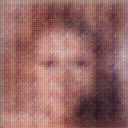
\includegraphics[width=150px]{500_fake_images/samples_5_283.png}%
\caption{A Man In A Suit And Tie Is Smiling}%
\end{figure}

%
\end{document}